
%(BEGIN_QUESTION)
% Copyright 2013, Tony R. Kuphaldt, released under the Creative Commons Attribution License (v 1.0)
% This means you may do almost anything with this work of mine, so long as you give me proper credit

This circuit uses two redundant pressure-actuated switches to sense the same fluid pressure.  If both switches are functioning properly, they should actuate at the same times and in the same ways.  Their combined effect controls power to a lamp to signify the process fluid pressure, an energized lamp for high pressure and a de-energized lamp for low pressure:

$$\includegraphics[width=15.5cm]{i03361x01.eps}$$

Construct a sentence using the conjunction ``AND'' to describe how the function of each pressure switch relates to the status of the lamp, choosing phrases from the bulleted list below:

\vskip 10pt

\centerline{\it If \underbar{\hskip 100pt} and \underbar{\hskip 100pt} then \underbar{\hskip 100pt}}

\begin{itemize}
\item{} PSH-1 closes when it senses high pressure
\item{} PSH-2 closes when it senses high pressure
\item{} PSH-1 opens when it senses low pressure
\item{} PSH-2 opens when it senses low pressure
\item{} PSH-1 remains open when it senses high pressure
\item{} PSH-2 remains open when it senses high pressure
\item{} PSH-1 remains closed when it senses low pressure
\item{} PSH-2 remains closed when it senses low pressure
\item{} The lamp will energize as it should
\item{} The lamp will remain energized when it should de-energize
\item{} The lamp will remain de-energized when it should energize
\item{} The lamp will de-energize as it should
\end{itemize}

\vskip 10pt

Next, construct another sentence from the bullet-list of phrases, this time using the conjunction ``OR'' instead of ``AND'':

\vskip 10pt

\centerline{\it If \underbar{\hskip 100pt} or \underbar{\hskip 100pt} then \underbar{\hskip 100pt}}

\vskip 10pt

Lastly, explain how this exercise in sentence construction might be helpful when deciding how to calculate probabilities in a system based on component dependability and unreliability (PFD).

\vskip 10pt

\underbar{file i03361}
%(END_QUESTION)





%(BEGIN_ANSWER)

Many correct statements are possible, using both AND and OR conjunctions.  Here are some samples:

\vskip 10pt

{\it If \underbar{PSH-1 closes when it senses high pressure} and \underbar{PSH-2 closes when it senses high pressure} then \underbar{the lamp will energize as it should}}

\vskip 10pt

{\it If \underbar{PSH-1 remains open when it senses high pressure} and \underbar{PSH-2 closes when it senses high pressure} then \underbar{the lamp will remain de-energized when it should energize}}

\vskip 10pt

{\it If \underbar{PSH-1 opens when it senses low pressure} or \underbar{PSH-2 opens when it senses low pressure} then \underbar{the lamp will de-energize as it should}}

\vskip 10pt

Constructing accurate sentences describing the operation of the system reveals the proper Boolean operations to apply to known component probabilities, in order to calculate the probability of the end-result.  For example, if the probability that each switch will close when it senses a high pressure is 0.992, then the probability that the lamp will energize when it should is 0.992 $\times$ 0.992 = 0.984064.

%(END_ANSWER)





%(BEGIN_NOTES)


%INDEX% Mathematics, probability: complementation
%INDEX% Safety, system reliability: probability of failure on demand (PFD)

%(END_NOTES)


